\documentclass{article}
\usepackage[utf8]{inputenc}
\usepackage{makecell}
\usepackage{booktabs}
\usepackage{multirow}
\usepackage[left=2cm,right=2cm]{geometry}
\usepackage{graphicx}
\usepackage{caption}
\usepackage{subcaption}
\usepackage{longtable}
\usepackage[dvipsnames]{xcolor}


\graphicspath{{figs/}}
\DeclareGraphicsExtensions{.png,.pdf}

\definecolor{color-bad}{rgb}{1, 0.9, 0.8}
\definecolor{color-very-bad}{rgb}{1, 0.7, 0.7}
\definecolor{color-abit}{rgb}{1, 1, 0.8}      % legacy, not used
\definecolor{color-good}{rgb}{1, 1, 1}     % this is white


\newcommand{\completeexample}[1]{%
  \textbf{\textit{\uline{\textcolor{color-very-bad}{\colorbox{color-bad}{#1}}}}}%
}
\newcommand{\orig}[1]{%
  \textbf{\textcolor{black}{\colorbox{color-good}{#1}}}%
}
\newcommand{\arxg}[1]{%
  \textnormal{\textcolor{black}{\colorbox{color-good}{#1}}}%
}
\newcommand{\arxb}[1]{%
  \textnormal{\textcolor{black}{\colorbox{color-bad}{#1}}}%
}
\newcommand{\arxvb}[1]{%
  \textnormal{\textcolor{black}{\colorbox{color-very-bad}{#1}}}%
}
\newcommand{\sdvg}[1]{%
  \textnormal{\textcolor{black}{\colorbox{color-good}{#1}}}%
}
\newcommand{\sdvb}[1]{%
  \textnormal{\textcolor{black}{\colorbox{color-bad}{#1}}}%
}
\newcommand{\sdvvb}[1]{%
  \textnormal{\textcolor{black}{\colorbox{color-very-bad}{#1}}}%
}
\newcommand{\sdxg}[1]{%
  \textnormal{\textcolor{black}{\colorbox{color-good}{#1}}}%
}
\newcommand{\sdxb}[1]{%
  \textnormal{\textcolor{black}{\colorbox{color-bad}{#1}}}%
}
\newcommand{\sdxvb}[1]{%
  \textnormal{\textcolor{black}{\colorbox{color-very-bad}{#1}}}%
}



\begin{document}

      \begin{table}
      \begin{center}
      \begin{small}
      \begin{tabular}{lllllll}
      \toprule
        & \multirow{2}{*}{\makecell[l]{\textbf{Commuting}\\\textbf{Modes}}}
          & \multicolumn{5}{l}{\textbf{Commuting from school}} \\ \cline{3-7}
        & & Car & Public & Wheels & Walk & Total \\
      \midrule
        \multirow{5}{*}{\makecell[l]{\textbf{Commuting}\\\textbf{to school}}}
    & Car      &  \makecell[l]{\textbf{58 (8.1\%)} \\58 (8.1\%) \\53 (7.4\%) \\20 (2.8\%)}      &  \makecell[l]{\textbf{54 (7.6\%)} \\54 (7.6\%) \\50 (7.0\%) \\48 (6.7\%)}      &  \makecell[l]{\textbf{1 (0.1\%)} \\0 (0.0\%) \\0 (0.0\%) \\15 (2.1\%)}      &  \makecell[l]{\textbf{57 (8.0\%)} \\57 (8.0\%) \\61 (8.6\%) \\94 (13.2\%)}      & \makecell[l]{\textbf{170 (23.8\%)} \\169 (23.7\%) \\164 (23.0\%) \\177 (24.8\%) \\} \\ \cline{2-7}
& Public      &  \makecell[l]{\textbf{10 (1.4\%)} \\8 (1.1\%) \\2 (0.3\%) \\37 (5.2\%)}      &  \makecell[l]{\textbf{190 (26.6\%)} \\194 (27.2\%) \\206 (28.9\%) \\69 (9.7\%)}      &  \makecell[l]{\textbf{0 (0.0\%)} \\0 (0.0\%) \\0 (0.0\%) \\34 (4.8\%)}      &  \makecell[l]{\textbf{30 (4.2\%)} \\30 (4.2\%) \\26 (3.6\%) \\81 (11.4\%)}      & \makecell[l]{\textbf{230 (32.3\%)} \\232 (32.5\%) \\234 (32.8\%) \\221 (31.0\%) \\} \\ \cline{2-7}
& Wheels      &  \makecell[l]{\textbf{0 (0.0\%)} \\0 (0.0\%) \\0 (0.0\%) \\20 (2.8\%)}      &  \makecell[l]{\textbf{0 (0.0\%)} \\0 (0.0\%) \\0 (0.0\%) \\23 (3.2\%)}      &  \makecell[l]{\textbf{27 (3.8\%)} \\29 (4.1\%) \\24 (3.4\%) \\13 (1.8\%)}      &  \makecell[l]{\textbf{7 (1.0\%)} \\6 (0.8\%) \\6 (0.8\%) \\40 (5.6\%)}      & \makecell[l]{\textbf{34 (4.8\%)} \\35 (4.9\%) \\30 (4.2\%) \\96 (13.5\%) \\} \\ \cline{2-7}
& Walk      &  \makecell[l]{\textbf{3 (0.4\%)} \\0 (0.0\%) \\0 (0.0\%) \\18 (2.5\%)}      &  \makecell[l]{\textbf{1 (0.1\%)} \\0 (0.0\%) \\0 (0.0\%) \\70 (9.8\%)}      &  \makecell[l]{\textbf{0 (0.0\%)} \\0 (0.0\%) \\1 (0.1\%) \\35 (4.9\%)}      &  \makecell[l]{\textbf{275 (38.6\%)} \\279 (39.1\%) \\283 (39.7\%) \\96 (13.5\%)}      & \makecell[l]{\textbf{279 (39.1\%)} \\279 (39.1\%) \\284 (39.8\%) \\219 (30.7\%) \\} \\ \cline{2-7}
& Total      & \makecell[l]{\textbf{71 (10.0\%)} \\66 (9.3\%) \\55 (7.7\%) \\95 (13.3\%) \\}      & \makecell[l]{\textbf{245 (34.4\%)} \\248 (34.8\%) \\256 (35.9\%) \\210 (29.5\%) \\}      & \makecell[l]{\textbf{28 (3.9\%)} \\29 (4.1\%) \\25 (3.5\%) \\97 (13.6\%) \\}      & \makecell[l]{\textbf{369 (51.8\%)} \\372 (52.2\%) \\376 (52.7\%) \\311 (43.6\%) \\}      & \makecell[l]{\textbf{713 (100.0\%)} \\715 (100.3\%)  \\712 (99.9\%)  \\713 (100.0\%)  \\} \\ 

      \bottomrule
      \end{tabular}
      \end{small}
      \caption{Table 1 from the paper showing the counts and percentages for the original data and the three anonymization methods. Each group of four presents the data in order of Original (bold), SynDiffix, ARX, and SDV.}
      \label{tab:table1}
      \end{center}
      \end{table}
    

      \begin{table}
      \begin{center}
      \begin{small}
      \begin{tabular}{lllll}
      \toprule
        \multirow{2}{*}{\makecell[l]{\textbf{Commuting}\\\textbf{group}}}
          & \multicolumn{2}{l}{\textbf{From home to school}}
          & \multicolumn{2}{l}{\textbf{From school to home}} \\ \cline{2-3} \cline{4-5}
          & \textbf{N (\%)} & \textbf{Distance (IQR)} & \textbf{N (\%)} & \textbf{Distance (IQR)} \\
      \midrule
    Car      &  \makecell[l]{\textbf{170 (24\%)} \\169 (24\%) \\182 (26\%) \\177 (25\%) \\}      &  \makecell[l]{\textbf{3133 (3945)} \\3532 (4155) \\3758 (3915) \\7602 (8467) \\}      &  \makecell[l]{\textbf{71 (10\%)} \\70 (10\%) \\58 (8\%) \\95 (13\%) \\}      &  \makecell[l]{\textbf{3615 (3896)} \\2615 (4607) \\3910 (3800) \\3934 (7362) \\} \\ \cline{2-5}
Public      &  \makecell[l]{\textbf{230 (32\%)} \\232 (33\%) \\212 (30\%) \\221 (31\%) \\}      &  \makecell[l]{\textbf{4782 (4296)} \\4676 (3960) \\4973 (4193) \\5690 (8320) \\}      &  \makecell[l]{\textbf{245 (34\%)} \\245 (34\%) \\252 (35\%) \\210 (29\%) \\}      &  \makecell[l]{\textbf{4996 (4033)} \\5296 (3600) \\5140 (3686) \\2249 (5174) \\} \\ \cline{2-5}
Wheels      &  \makecell[l]{\textbf{34 (5\%)} \\36 (5\%) \\31 (4\%) \\96 (13\%) \\}      &  \makecell[l]{\textbf{1366 (2211)} \\1097 (1254) \\1356 (1378) \\6671 (8472) \\}      &  \makecell[l]{\textbf{28 (4\%)} \\30 (4\%) \\14 (2\%) \\97 (14\%) \\}      &  \makecell[l]{\textbf{1444 (2369)} \\1236 (2263) \\2235 (3245) \\2741 (5282) \\} \\ \cline{2-5}
Walk      &  \makecell[l]{\textbf{279 (39\%)} \\279 (39\%) \\278 (39\%) \\219 (31\%) \\}      &  \makecell[l]{\textbf{799 (789)} \\789 (797) \\805 (795) \\5498 (8697) \\}      &  \makecell[l]{\textbf{369 (52\%)} \\368 (52\%) \\379 (53\%) \\311 (44\%) \\}      &  \makecell[l]{\textbf{973 (1043)} \\952 (996) \\954 (1062) \\2374 (6068) \\} \\ \cline{2-5}
      Total       & \makecell[l]{\textbf{713 (100\%)} \\716 (100\%) \\703 (99\%) \\713 (100\%) \\} &       & \makecell[l]{\textbf{713 (100\%)} \\713 (100\%) \\703 (99\%) \\713 (100\%) \\} & \\ 

      \bottomrule
      \end{tabular}
      \end{small}
      \caption{Table 2 from the original paper showing the counts and distances in meters (median and IQR) for the original data and the three anonymization methods. Each group of four presents the data in order of Original (bold), SynDiffix, ARX, and SDV. Note that the original distances median and IQR don't perfectly match those of the original Table 2 because of differences in the way median and IQR were calculated (Python versus R).}
      \label{tab:table2}
      \end{center}
      \end{table}
    

      \setlength{\fboxsep}{0pt}
      \begin{table}
      \begin{center}
      \begin{small}
      \begin{tabular}{lllll}
      \toprule
        \textbf{Variables}
          & \multicolumn{4}{l}{\textbf{Adjusted model}} \\ \cline{2-5}
        & \multicolumn{2}{l}{\textbf{From home to school}} 
          & \multicolumn{2}{l}{\textbf{From school to home}} \\ \cline{2-3} \cline{4-5}
        & \textbf{Coefficient} & \textbf{95\% CI} & \textbf{Coefficient} & \textbf{95\% CI} \\
      \midrule
    \textbf{Constant}    &  \makecell[l]{\orig{36.42}\orig{***} \\\arxg{33.19}\arxg{***} \\\sdvg{56.08}\sdvg{***} \\\sdxg{27.94}\sdxg{***} \\}   &  \makecell[l]{\orig{(28.17}, \orig{44.67)} \\\arxg{(25.82}, \arxg{40.56)} \\\sdvg{(45.07}, \sdvg{67.09)} \\\sdxg{(20.74}, \sdxg{35.14)} \\}   &  \makecell[l]{\orig{36.63}\orig{***} \\\arxg{35.36}\arxg{***} \\\sdvg{49.18}\sdvg{***} \\\sdxg{32.89}\sdxg{***} \\}   &  \makecell[l]{\orig{(29.11}, \orig{44.15)} \\\arxg{(28.65}, \arxg{42.07)} \\\sdvg{(40.44}, \sdvg{57.91)} \\\sdxg{(26.25}, \sdxg{39.54)} \\} \\ 
\multicolumn{5}{l}{\textbf{Commuting group}} \\ 
\quad Car    &  \makecell[l]{\orig{-6.49}\orig{\phantom{***}} \\\arxg{-7.28}\arxg{\phantom{***}} \\\sdvg{-9.17}\sdvg{\phantom{***}} \\\sdxg{-2.18}\sdxg{\phantom{***}} \\}   &  \makecell[l]{\orig{(-15.92}, \orig{2.94)} \\\arxg{(-15.49}, \arxg{0.92)} \\\sdvg{(-21.3}, \sdvg{2.95)} \\\sdxg{(-9.25}, \sdxg{4.88)} \\}   &  \makecell[l]{\orig{-15.13}\orig{*\phantom{**}} \\\arxg{-17.72}\arxg{**\phantom{*}} \\\sdvg{2.4}\sdvvb{\phantom{***}} \\\sdxg{-12.67}\sdxg{*\phantom{**}} \\}   &  \makecell[l]{\orig{(-26.88}, \orig{-3.39)} \\\arxg{(-29.65}, \arxg{-5.8)} \\\sdvg{(-6.44}, \sdvg{11.24)} \\\sdxg{(-22.82}, \sdxg{-2.52)} \\} \\ 
& & & & \\ 
\quad Public    &  \makecell[l]{\orig{-0.08}\orig{\phantom{***}} \\\arxg{3.21}\arxg{\phantom{***}} \\\sdvg{-6.17}\sdvg{\phantom{***}} \\\sdxg{-0.15}\sdxg{\phantom{***}} \\}   &  \makecell[l]{\orig{(-9.06}, \orig{8.9)} \\\arxg{(-4.59}, \arxg{11.01)} \\\sdvg{(-16.67}, \sdvg{4.32)} \\\sdxg{(-6.37}, \sdxg{6.07)} \\}   &  \makecell[l]{\orig{-3.19}\orig{\phantom{***}} \\\arxg{-4.08}\arxg{\phantom{***}} \\\sdvg{-2.57}\sdvg{\phantom{***}} \\\sdxg{8.71}\sdxvb{**\phantom{*}} \\}   &  \makecell[l]{\orig{(-11.27}, \orig{4.88)} \\\arxg{(-10.99}, \arxg{2.84)} \\\sdvg{(-9.06}, \sdvg{3.92)} \\\sdxg{(2.72}, \sdxg{14.71)} \\} \\ 
& & & & \\ 
\quad Wheels    &  \makecell[l]{\orig{3.0}\orig{\phantom{***}} \\\arxg{3.88}\arxg{\phantom{***}} \\\sdvg{-8.69}\sdvg{\phantom{***}} \\\sdxg{3.23}\sdxg{\phantom{***}} \\}   &  \makecell[l]{\orig{(-16.24}, \orig{22.25)} \\\arxg{(-11.83}, \arxg{19.58)} \\\sdvg{(-23.52}, \sdvg{6.14)} \\\sdxg{(-10.68}, \sdxg{17.13)} \\}   &  \makecell[l]{\orig{15.66}\orig{\phantom{***}} \\\arxg{17.16}\arxg{\phantom{***}} \\\sdvg{1.48}\sdvg{\phantom{***}} \\\sdxg{10.7}\sdxg{\phantom{***}} \\}   &  \makecell[l]{\orig{(-4.09}, \orig{35.41)} \\\arxg{(-4.9}, \arxg{39.22)} \\\sdvg{(-7.47}, \sdvg{10.44)} \\\sdxg{(-3.6}, \sdxg{24.99)} \\} \\ 
\quad Walk (ref) & & & & \\ 
\multicolumn{5}{l}{\textbf{Interaction Commuting group x Distance}} \\ 
\quad Car x Distance    &  \makecell[l]{\orig{0.58}\orig{\phantom{***}} \\\arxg{0.79}\arxvb{**\phantom{*}} \\\sdvg{0.35}\sdvg{\phantom{***}} \\\sdxg{0.42}\sdxg{\phantom{***}} \\}   &  \makecell[l]{\orig{(-0.04}, \orig{1.2)} \\\arxg{(0.24}, \arxg{1.34)} \\\sdvg{(-0.35}, \sdvg{1.06)} \\\sdxg{(-0.08}, \sdxg{0.91)} \\}   &  \makecell[l]{\orig{1.25}\orig{**\phantom{*}} \\\arxg{1.38}\arxg{**\phantom{*}} \\\sdvg{-0.28}\sdvvb{\phantom{***}} \\\sdxg{2.06}\sdxg{***} \\}   &  \makecell[l]{\orig{(0.34}, \orig{2.17)} \\\arxg{(0.44}, \arxg{2.33)} \\\sdvg{(-0.94}, \sdvg{0.37)} \\\sdxg{(1.19}, \sdxg{2.93)} \\} \\ 
& & & & \\ 
\quad Public x Distance    &  \makecell[l]{\orig{0.06}\orig{\phantom{***}} \\\arxg{-0.04}\arxg{\phantom{***}} \\\sdvg{0.04}\sdvg{\phantom{***}} \\\sdxg{0.26}\sdxg{\phantom{***}} \\}   &  \makecell[l]{\orig{(-0.49}, \orig{0.61)} \\\arxg{(-0.52}, \arxg{0.45)} \\\sdvg{(-0.48}, \sdvg{0.56)} \\\sdxg{(-0.13}, \sdxg{0.65)} \\}   &  \makecell[l]{\orig{0.33}\orig{\phantom{***}} \\\arxg{0.37}\arxg{\phantom{***}} \\\sdvg{0.38}\sdvg{\phantom{***}} \\\sdxg{0.03}\sdxg{\phantom{***}} \\}   &  \makecell[l]{\orig{(-0.21}, \orig{0.88)} \\\arxg{(-0.1}, \arxg{0.84)} \\\sdvg{(-0.06}, \sdvg{0.82)} \\\sdxg{(-0.39}, \sdxg{0.45)} \\} \\ 
& & & & \\ 
\quad Wheels x Distance    &  \makecell[l]{\orig{-0.09}\orig{\phantom{***}} \\\arxg{0.08}\arxg{\phantom{***}} \\\sdvg{0.09}\sdvg{\phantom{***}} \\\sdxg{0.19}\sdxg{\phantom{***}} \\}   &  \makecell[l]{\orig{(-1.79}, \orig{1.62)} \\\arxg{(-1.32}, \arxg{1.48)} \\\sdvg{(-0.88}, \sdvg{1.07)} \\\sdxg{(-1.07}, \sdxg{1.44)} \\}   &  \makecell[l]{\orig{-1.15}\orig{\phantom{***}} \\\arxg{-1.41}\arxg{\phantom{***}} \\\sdvg{-0.04}\sdvg{\phantom{***}} \\\sdxg{-0.13}\sdxg{\phantom{***}} \\}   &  \makecell[l]{\orig{(-2.89}, \orig{0.6)} \\\arxg{(-3.35}, \arxg{0.53)} \\\sdvg{(-0.75}, \sdvg{0.66)} \\\sdxg{(-1.36}, \sdxg{1.11)} \\} \\ 
& & & & \\ 
\quad Walk x Distance    &  \makecell[l]{\orig{-0.02}\orig{\phantom{***}} \\\arxg{0.17}\arxg{\phantom{***}} \\\sdvg{-0.63}\sdvg{\phantom{***}} \\\sdxg{0.17}\sdxg{\phantom{***}} \\}   &  \makecell[l]{\orig{(-0.62}, \orig{0.58)} \\\arxg{(-0.33}, \arxg{0.68)} \\\sdvg{(-1.28}, \sdvg{0.02)} \\\sdxg{(-0.24}, \sdxg{0.58)} \\}   &  \makecell[l]{\orig{0.03}\orig{\phantom{***}} \\\arxg{-0.04}\arxg{\phantom{***}} \\\sdvg{-0.08}\sdvg{\phantom{***}} \\\sdxg{0.66}\sdxvb{***} \\}   &  \makecell[l]{\orig{(-0.42}, \orig{0.48)} \\\arxg{(-0.42}, \arxg{0.34)} \\\sdvg{(-0.44}, \sdvg{0.28)} \\\sdxg{(0.3}, \sdxg{1.02)} \\} \\ 

      \bottomrule
      {\footnotesize * p $\leq$ 0.05, \quad** p $\leq$ 0.01, \quad*** p $\leq$ 0.001}
      \end{tabular}
      \end{small}
      \caption{Part 1 (of 2) of the original paper's Table 3 showing the parameters (regression coefficients) of the linear model for prediction of VO2max by group and distance. \colorbox{color-very-bad}{Red} shading indcates that the anonymized entry is non-significant where the original data is significant or vice versa. Each group of four presents the data in order of Original (bold), ARX, SDV, and SynDiffix. 
      }
      \label{tab:table3a}
      \end{center}
      \end{table}
      \setlength{\fboxsep}{3pt}
    

      \setlength{\fboxsep}{0pt}
      \begin{table}
      \begin{center}
      \begin{small}
      \begin{tabular}{lllll}
      \toprule
        \textbf{Variables}
          & \multicolumn{4}{l}{\textbf{Adjusted model}} \\ \cline{2-5}
        & \multicolumn{2}{l}{\textbf{From home to school}} 
          & \multicolumn{2}{l}{\textbf{From school to home}} \\ \cline{2-3} \cline{4-5}
        & \textbf{Coefficient} & \textbf{95\% CI} & \textbf{Coefficient} & \textbf{95\% CI} \\
      \midrule
    \textbf{Gender} & & & & \\ 
\quad Males    &  \makecell[l]{\orig{7.97}\orig{***} \\\arxg{8.19}\arxg{***} \\\sdvg{0.29}\sdvvb{\phantom{***}} \\\sdxg{7.27}\sdxg{***} \\}   &  \makecell[l]{\orig{(6.75}, \orig{9.19)} \\\arxg{(7.2}, \arxg{9.18)} \\\sdvg{(-1.66}, \sdvg{2.25)} \\\sdxg{(6.11}, \sdxg{8.44)} \\}   &  \makecell[l]{\orig{7.58}\orig{***} \\\arxg{7.45}\arxg{***} \\\sdvg{-0.36}\sdvvb{\phantom{***}} \\\sdxg{8.26}\sdxg{***} \\}   &  \makecell[l]{\orig{(6.52}, \orig{8.63)} \\\arxg{(6.6}, \arxg{8.29)} \\\sdvg{(-1.99}, \sdvg{1.27)} \\\sdxg{(7.31}, \sdxg{9.2)} \\} \\ 
\quad Females (ref) & & & & \\ 
\multicolumn{5}{l}{\textbf{Interaction Commuting group x Gender}} \\ 
\quad Car x Gender    &  \makecell[l]{\orig{-2.2}\orig{*\phantom{**}} \\\arxg{-2.32}\arxg{**\phantom{*}} \\\sdvg{-2.75}\sdvvb{\phantom{***}} \\\sdxg{-0.35}\sdxvb{\phantom{***}} \\}   &  \makecell[l]{\orig{(-4.16}, \orig{-0.24)} \\\arxg{(-3.86}, \arxg{-0.77)} \\\sdvg{(-5.66}, \sdvg{0.16)} \\\sdxg{(-2.17}, \sdxg{1.48)} \\}   &  \makecell[l]{\orig{-2.63}\orig{*\phantom{**}} \\\arxg{-2.3}\arxg{*\phantom{**}} \\\sdvg{0.41}\sdvvb{\phantom{***}} \\\sdxg{-4.21}\sdxg{**\phantom{*}} \\}   &  \makecell[l]{\orig{(-5.23}, \orig{-0.03)} \\\arxg{(-4.59}, \arxg{-0.01)} \\\sdvg{(-2.97}, \sdvg{3.78)} \\\sdxg{(-6.97}, \sdxg{-1.44)} \\} \\ 
& & & & \\ 
\quad Public x Males    &  \makecell[l]{\orig{-2.0}\orig{*\phantom{**}} \\\arxg{-2.56}\arxg{***} \\\sdvg{-1.69}\sdvvb{\phantom{***}} \\\sdxg{-0.5}\sdxvb{\phantom{***}} \\}   &  \makecell[l]{\orig{(-3.81}, \orig{-0.2)} \\\arxg{(-4.05}, \arxg{-1.07)} \\\sdvg{(-4.46}, \sdvg{1.07)} \\\sdxg{(-2.16}, \sdxg{1.16)} \\}   &  \makecell[l]{\orig{-1.35}\orig{\phantom{***}} \\\arxg{-1.53}\arxvb{*\phantom{**}} \\\sdvg{-2.18}\sdvg{\phantom{***}} \\\sdxg{-1.88}\sdxvb{*\phantom{**}} \\}   &  \makecell[l]{\orig{(-2.99}, \orig{0.3)} \\\arxg{(-2.83}, \arxg{-0.22)} \\\sdvg{(-4.77}, \sdvg{0.4)} \\\sdxg{(-3.35}, \sdxg{-0.41)} \\} \\ 
& & & & \\ 
\quad Wheels x Males    &  \makecell[l]{\orig{-1.95}\orig{\phantom{***}} \\\arxg{-4.06}\arxg{\phantom{***}} \\\sdvg{-0.17}\sdvg{\phantom{***}} \\\sdxg{0.05}\sdxg{\phantom{***}} \\}   &  \makecell[l]{\orig{(-7.49}, \orig{3.6)} \\\arxg{(-10.16}, \arxg{2.05)} \\\sdvg{(-3.71}, \sdvg{3.38)} \\\sdxg{(-3.38}, \sdxg{3.47)} \\}   &  \makecell[l]{\orig{-3.09}\orig{\phantom{***}} \\\arxg{nan}\arxg{\phantom{***}} \\\sdvg{0.16}\sdvg{\phantom{***}} \\\sdxg{nan}\sdxg{\phantom{***}} \\}   &  \makecell[l]{\orig{(-9.31}, \orig{3.12)} \\\arxg{(nan}, \arxg{nan)} \\\sdvg{(-3.25}, \sdvg{3.56)} \\\sdxg{(nan}, \sdxg{nan)} \\} \\ 
\quad Walk x Males (ref) & & & & \\ 
\textbf{Covariates} & & & & \\ 
\quad MVPA    &  \makecell[l]{\orig{0.08}\orig{***} \\\arxg{0.08}\arxg{***} \\\sdvg{-0.06}\sdvg{**\phantom{*}} \\\sdxg{0.17}\sdxg{***} \\}   &  \makecell[l]{\orig{(0.03}, \orig{0.12)} \\\arxg{(0.04}, \arxg{0.12)} \\\sdvg{(-0.11}, \sdvg{-0.02)} \\\sdxg{(0.13}, \sdxg{0.22)} \\}   &  \makecell[l]{\orig{0.07}\orig{***} \\\arxg{0.07}\arxg{***} \\\sdvg{-0.06}\sdvg{**\phantom{*}} \\\sdxg{0.14}\sdxg{***} \\}   &  \makecell[l]{\orig{(0.03}, \orig{0.11)} \\\arxg{(0.03}, \arxg{0.12)} \\\sdvg{(-0.11}, \sdvg{-0.01)} \\\sdxg{(0.09}, \sdxg{0.18)} \\} \\ 
& & & & \\ 
\quad Age    &  \makecell[l]{\orig{0.43}\orig{*\phantom{**}} \\\arxg{0.53}\arxg{**\phantom{*}} \\\sdvg{-0.11}\sdvvb{\phantom{***}} \\\sdxg{0.66}\sdxg{**\phantom{*}} \\}   &  \makecell[l]{\orig{(0.0}, \orig{0.85)} \\\arxg{(0.14}, \arxg{0.92)} \\\sdvg{(-0.64}, \sdvg{0.42)} \\\sdxg{(0.26}, \sdxg{1.06)} \\}   &  \makecell[l]{\orig{0.4}\orig{\phantom{***}} \\\arxg{0.55}\arxvb{**\phantom{*}} \\\sdvg{-0.08}\sdvg{\phantom{***}} \\\sdxg{-0.05}\sdxg{\phantom{***}} \\}   &  \makecell[l]{\orig{(-0.02}, \orig{0.82)} \\\arxg{(0.17}, \arxg{0.93)} \\\sdvg{(-0.61}, \sdvg{0.45)} \\\sdxg{(-0.43}, \sdxg{0.33)} \\} \\ 

      \bottomrule
      {\footnotesize * p $\leq$ 0.05, \quad** p $\leq$ 0.01, \quad*** p $\leq$ 0.001}
      \end{tabular}
      \end{small}
      \caption{Part 2 (of 2) of the original paper's Table 3 showing the parameters (regression coefficients) of the linear model for prediction of VO2max by group and distance. \colorbox{color-very-bad}{Red} shading indcates that the anonymized entry is non-significant where the original data is significant or vice versa. Each group of four presents the data in order of Original (bold), ARX, SDV, and SynDiffix. 
      }
      \label{tab:table3b}
      \end{center}
      \end{table}
      \setlength{\fboxsep}{3pt}
    

        \begin{figure}
        \begin{center}
        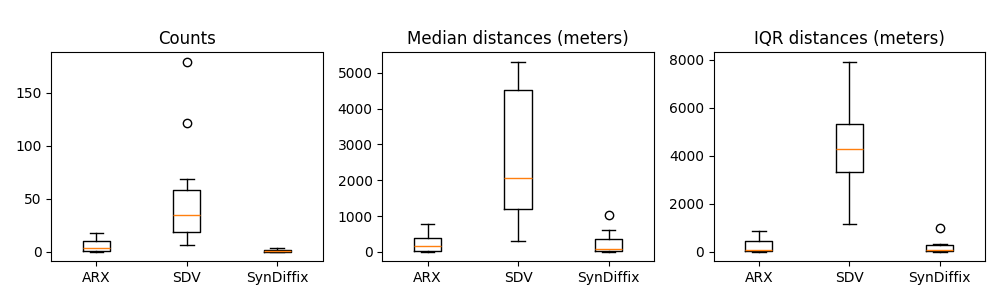
\includegraphics[width=0.85\linewidth]{abs_err_tab1_tab2}
        \caption{Absolute error of the three anonymization methods for the counts and distances in Tables~\ref{tab:table1} and \ref{tab:table2}.
        }
        \label{fig:abs_err_tab1_tab2}
        \end{center}
        \end{figure}
    


    \begin{figure}[htbp]
        \centering
        \begin{subfigure}[b]{0.48\textwidth}
            \centering
            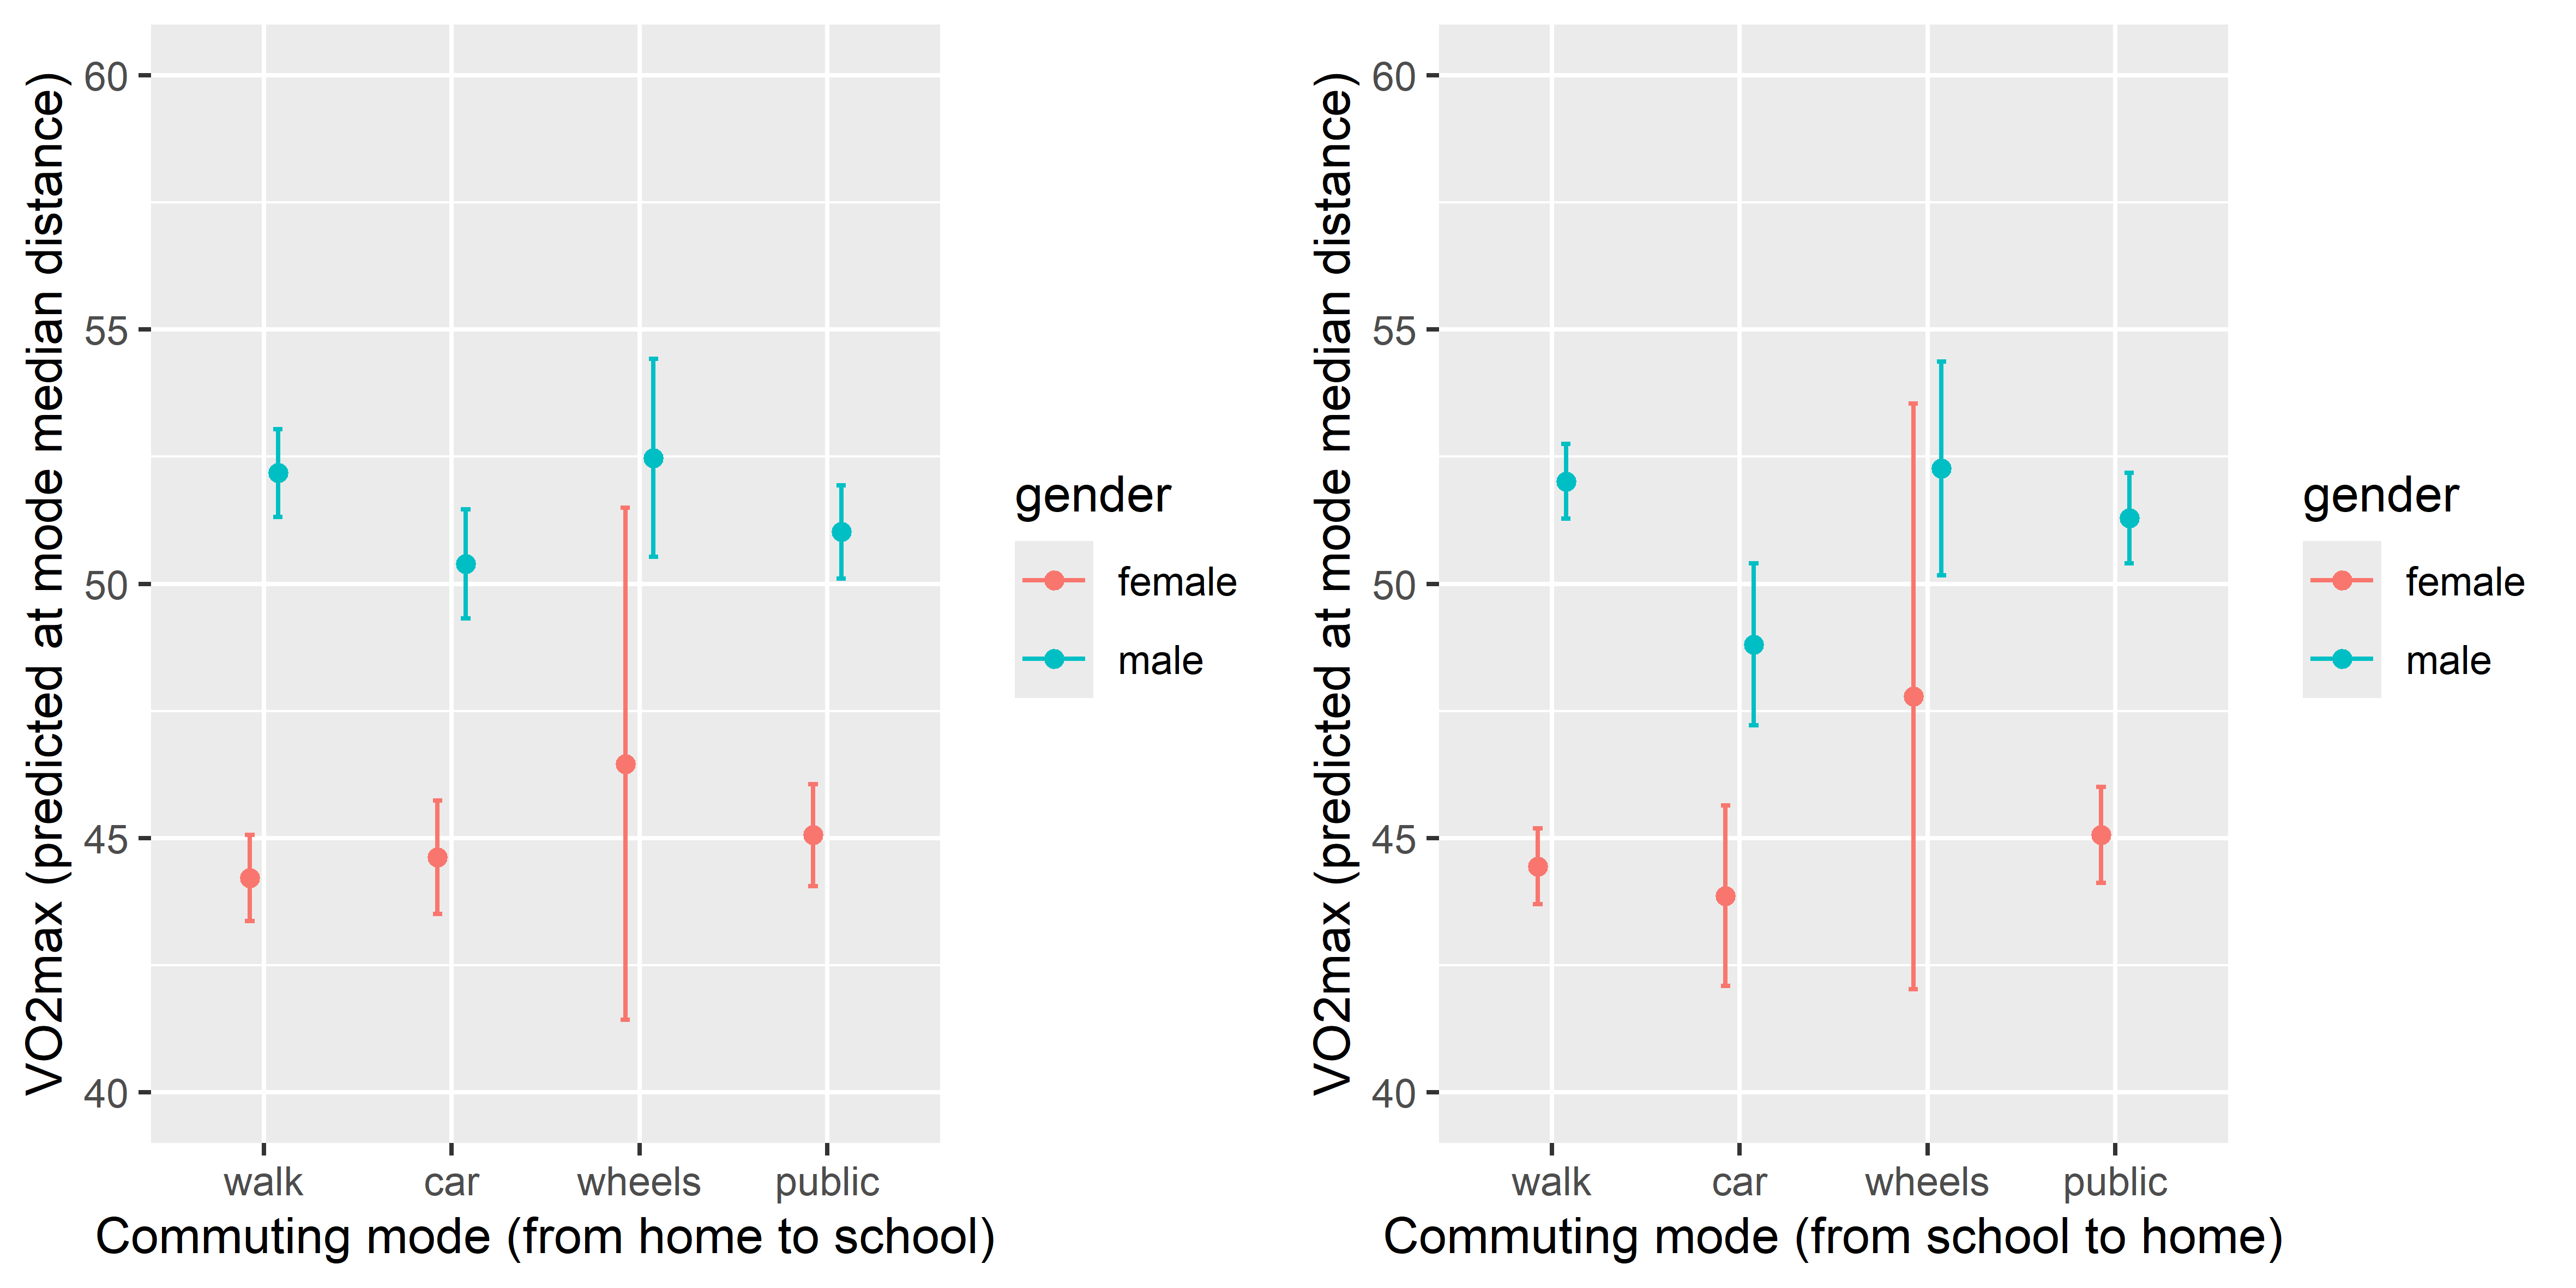
\includegraphics[width=\textwidth]{figs/r_orig_plot.png}
            \caption{Original Plot}
            \label{fig:r_orig_plot}
        \end{subfigure}
        \hspace{0.0\textwidth}
        \begin{subfigure}[b]{0.48\textwidth}
            \centering
            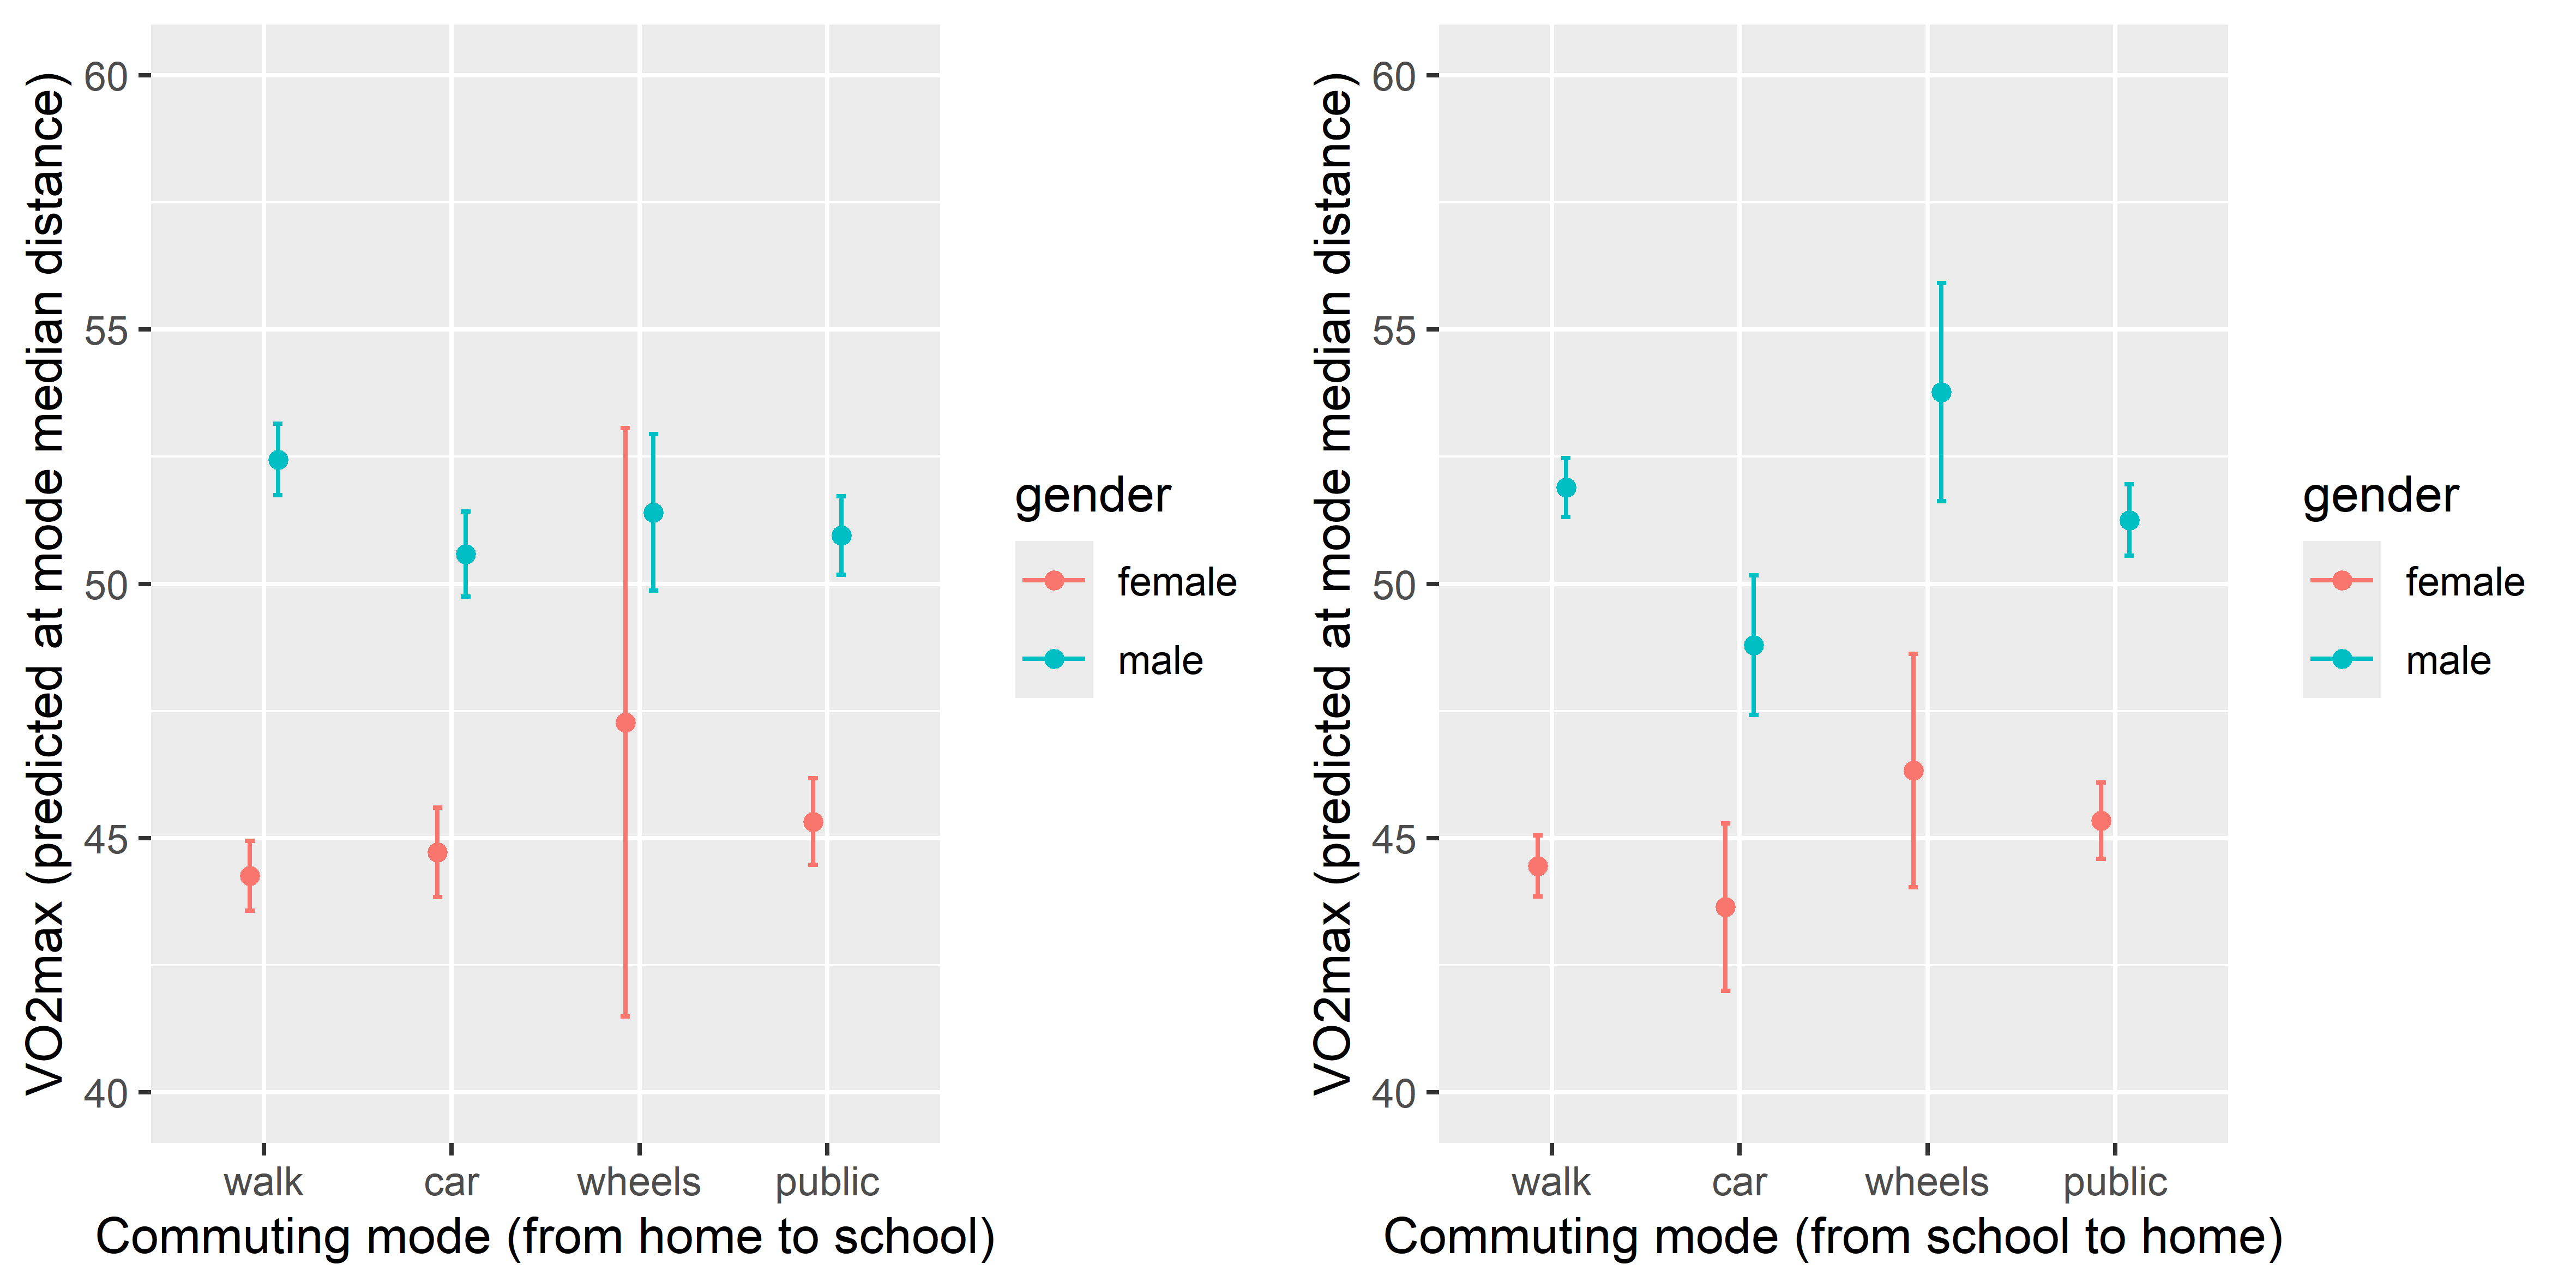
\includegraphics[width=\textwidth]{figs/r_arx_plot.png}
            \caption{ARX Plot}
            \label{fig:r_arx_plot}
        \end{subfigure}
        \vfill
        \begin{subfigure}[b]{0.48\textwidth}
            \centering
            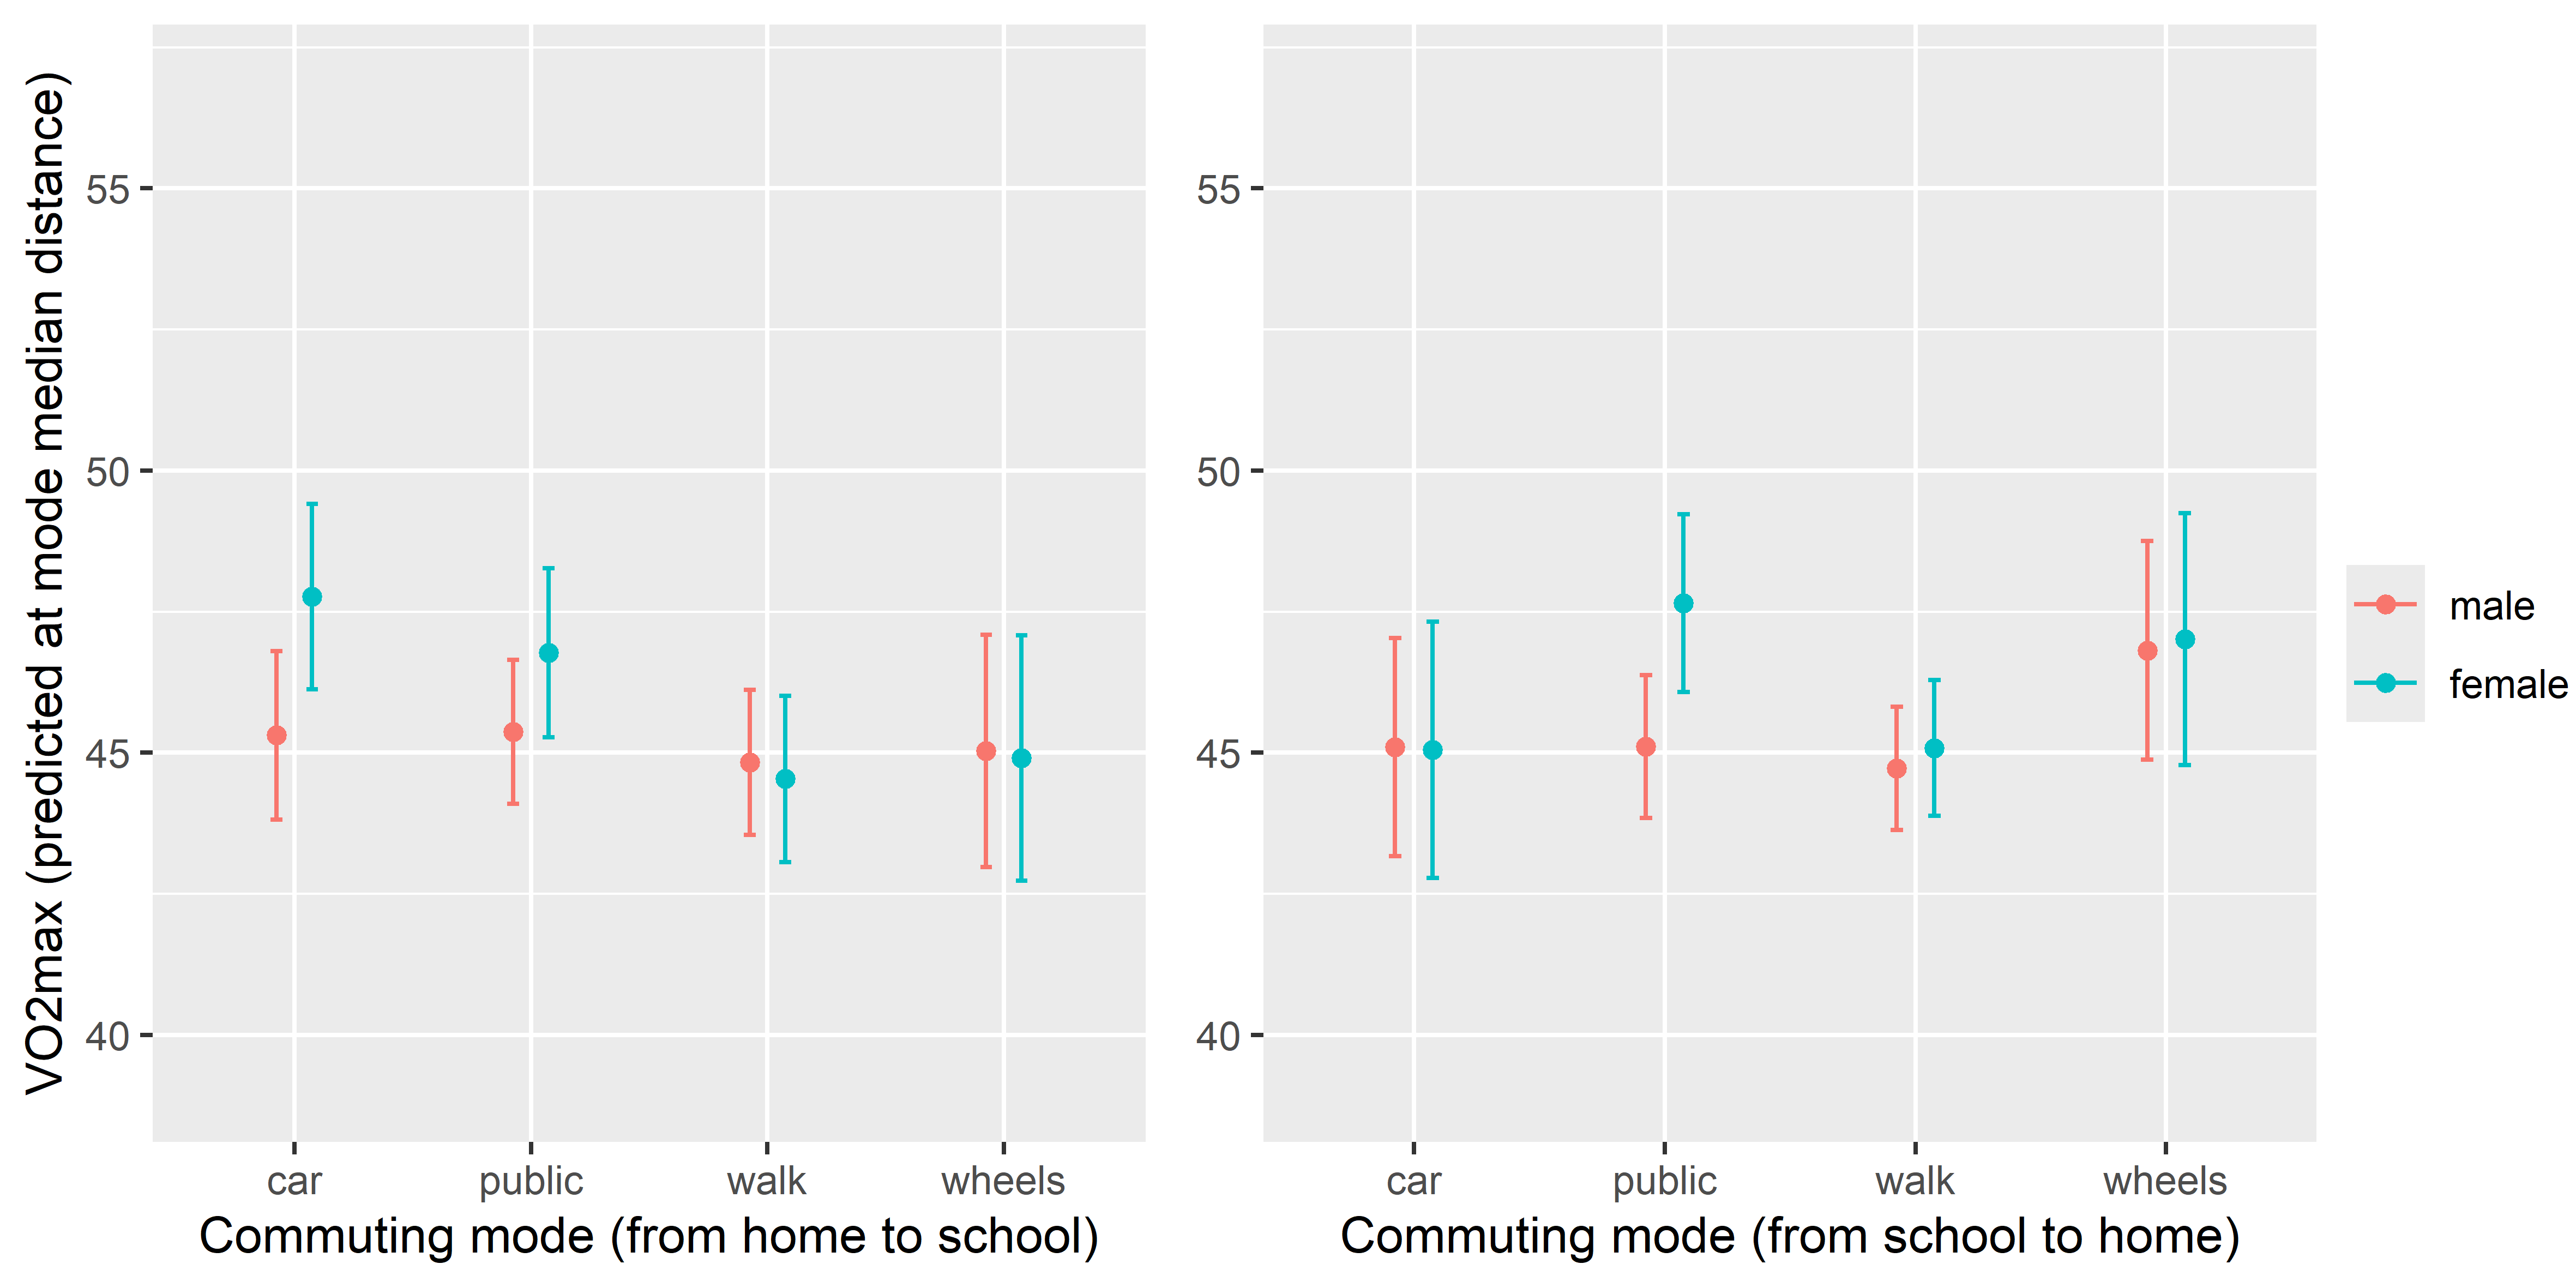
\includegraphics[width=\textwidth]{figs/r_sdv_plot.png}
            \caption{SDV Plot}
            \label{fig:r_sdv_plot}
        \end{subfigure}
        \hspace{0.0\textwidth}
        \begin{subfigure}[b]{0.48\textwidth}
            \centering
            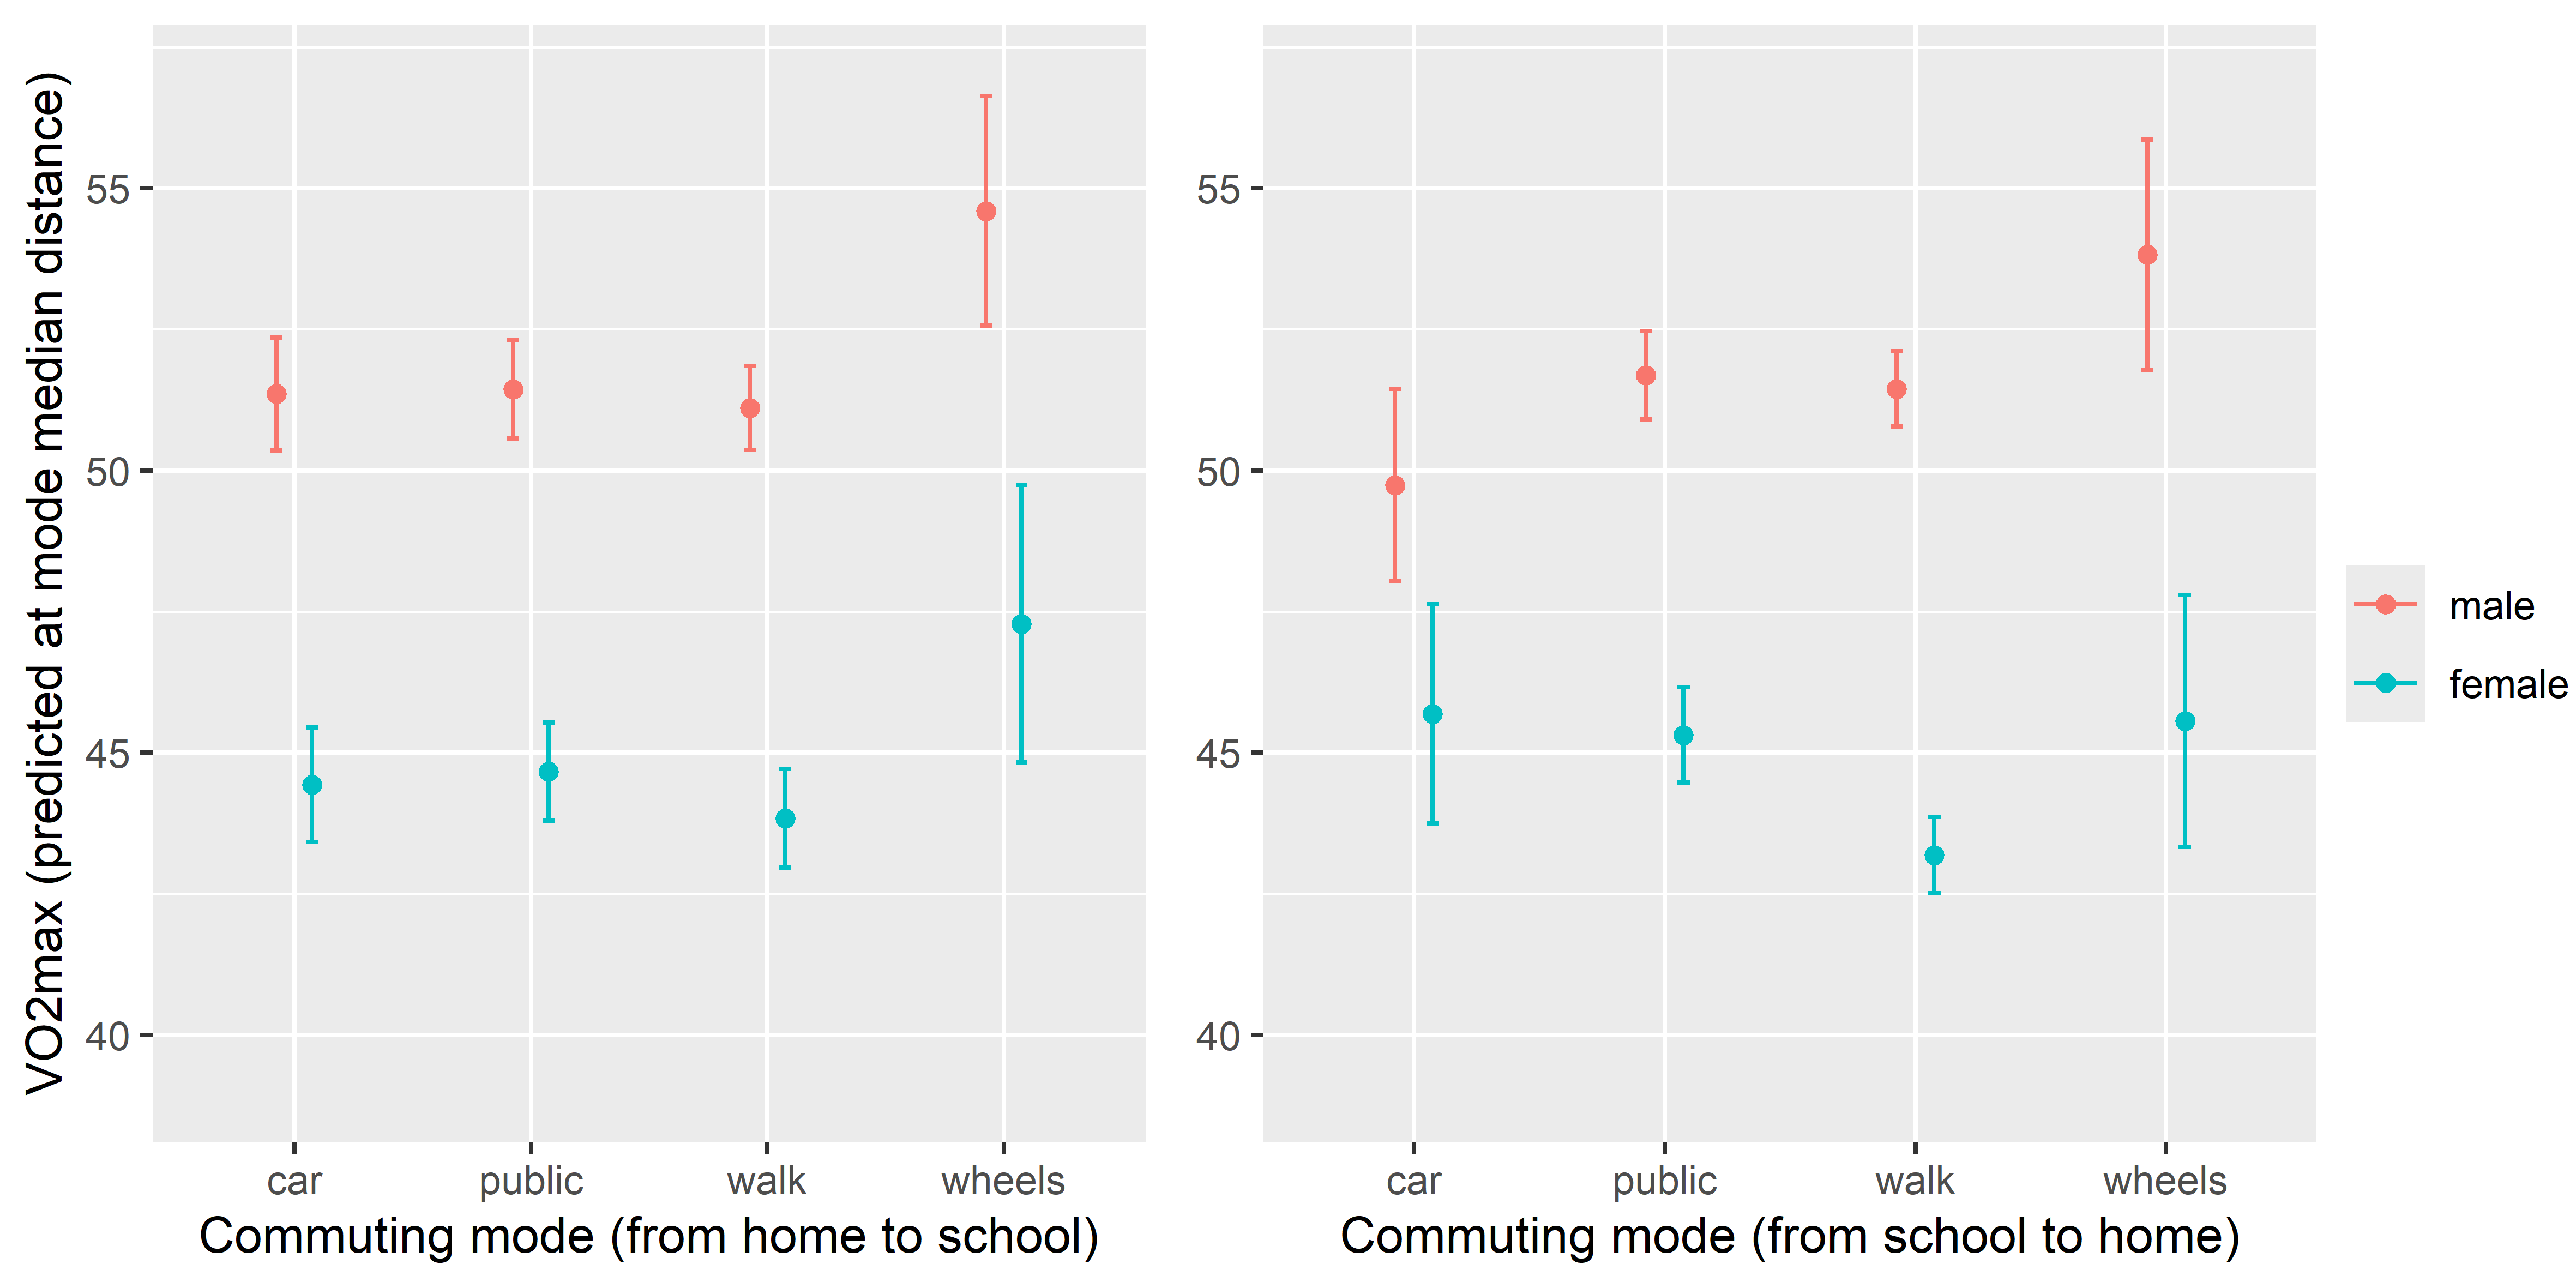
\includegraphics[width=\textwidth]{figs/r_sdx_plot.png}
            \caption{SynDiffix Plot}
            \label{fig:r_sdx_plot}
        \end{subfigure}

        \caption{Comparison of the VO2max data. Here we see that ARX matches very closely with the original data. SynDiffix is quite close for female, but for reasons I don't understand yet, does somewhat bad for the car commute for males. Otherwise, though SynDiffix is pretty good. SDV is again quite bad. What will be important is whether the correct conclusions can be drown from the data in spite of the error.
        }
        \label{fig:comparison_plots}
    \end{figure}

    

        \begin{figure}
        \begin{center}
        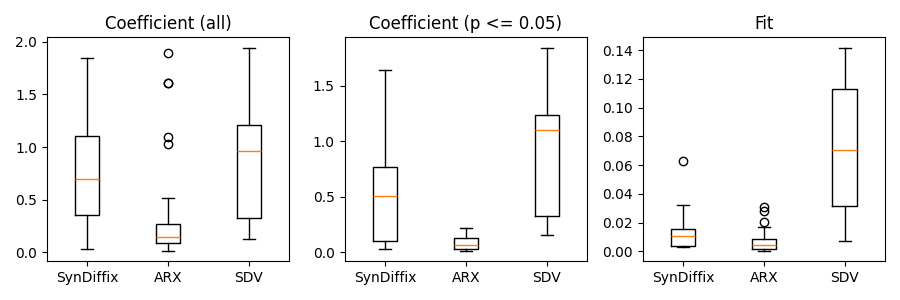
\includegraphics[width=0.65\linewidth]{norm_err_tab3_fig1}
        \caption{Normalized error for coefficients and fit for Figure~\ref{fig:comparison_plots}. This reflects the quality we see in Figure~\ref{fig:comparison_plots}. SynDiffix clearly has more error than ARX.
        }
        \end{center}
        \end{figure}
    

      \setlength{\fboxsep}{0pt}
      \begin{table}
      \begin{center}
      \begin{small}
      \begin{tabular}{llll}
      \toprule
        & ARX & SDV & SynDiffix \\
      \midrule
        Of the original 12 significant p-values, method is also significat  & 12 (100\%)  & 4 (33\%)  & 10 (83\%)  \\ 
    Of the original 16 insignificant p-values, method is also insignificat  & 13 (81\%)  & 16 (100\%)  & 13 (81\%)  \\ 
    Of the original 12 significant p-values, method matches  & 8 (67\%)  & 2 (17\%)  & 7 (58\%)  \\ 
    Of the original 12 significant p-values, method off by 1  & 3 (25\%)  & 2 (17\%)  & 3 (25\%)  \\ 
    Of the original 12 significant p-values, method off by 2  & 1 (8\%)  & 0 (0\%)  & 0 (0\%)  \\ 

      \bottomrule
      \end{tabular}
      \end{small}
      \caption{Error between each method's p-values and the original p-values. P-values are significant when $p \leq 0.05$. P-values are binned as $p \leq 0.001$, $0.001 < p \leq 0.01$, and $0.01 < p \leq 0.05$. Off by 1 means that the method's bin is one off from the original data's bin (both being significant). Off by 2 means that the method's bin is two off from the original data's bin.
      }
      \label{tab:p_table}
      \end{center}
      \end{table}
      \setlength{\fboxsep}{3pt}
    

        \begin{figure}
        \begin{center}
        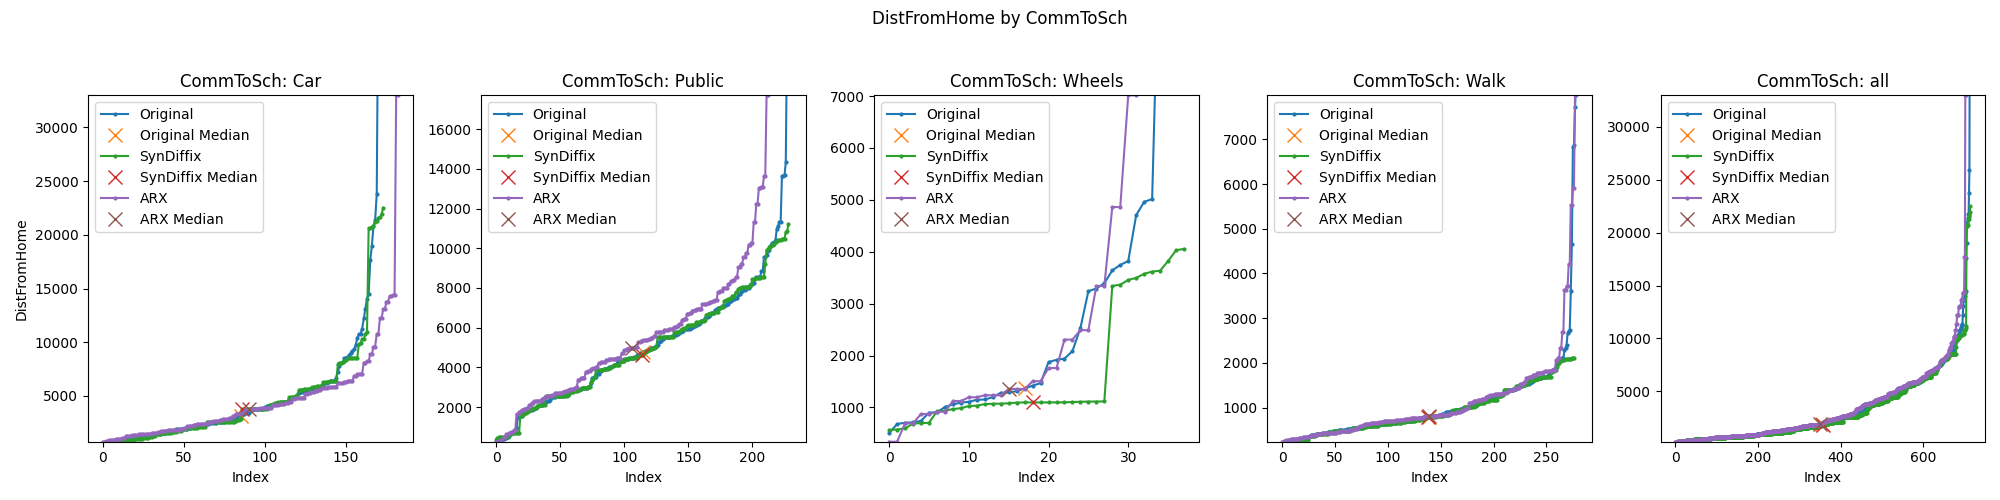
\includegraphics[width=1.0\linewidth]{median_plots}
        \caption{Distance from home distributions, by commuting type. Median distances marked with an X. I made this plot just to better understand where median distance errors were coming from for SynDiffix. There are two problems for SynDiffix. First, we adjust the "outlier" data points because they strictly speaking might break anonymity. Second, there are very few Wheels datapoints, and SynDiffix struggles with that. 
        }
        \label{fig:median_plots}
        \end{center}
        \end{figure}
    
\end{document}
